%*----------- SLIDE -------------------------------------------------------------
\begin{frame}[t]{Introdução}
    Sobre Marco A. dos Reis:
    \transboxout[duration=0.5]
    \begin{columns}
        \column{.1\textwidth}
        \column{.3\textwidth}
            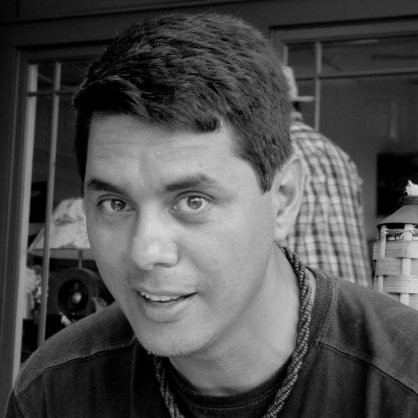
\includegraphics[width=1\textwidth]{marco.jpg}
        \column{.6\textwidth}
            \begin{itemize}
                \item Graduado em Engenharia Elétrico pela UFPR e Mestre em Engenharia de Produação pela UFSC
                \item É pesquisador do Instituto Brasileiro de Robótica, ação conjunta entre o Senai Cimatec e o Centro Alemão de Inteligência Artificial
                \item Professor convidado dos cursos de especialização em Automação, Controle e Robótica, e de Sistemas Elétricos de Potência do Senai CIMATEC
            \end{itemize}
    \end{columns}
 %*----------- notes
    \note[item]{Notes can help you to remember important information. Turn on the notes option.}
\end{frame}
%*----------- SLIDE -------------------------------------------------------------
\begin{frame}[c]{Justificativa}
    \begin{itemize}
        \item acompanhamento e monitoramento subaquático
        \item dificuldade de acesso para mergulhadores
        \item regiões de riscos para os mergulhadores
    \end{itemize}
    \begin{figure}
        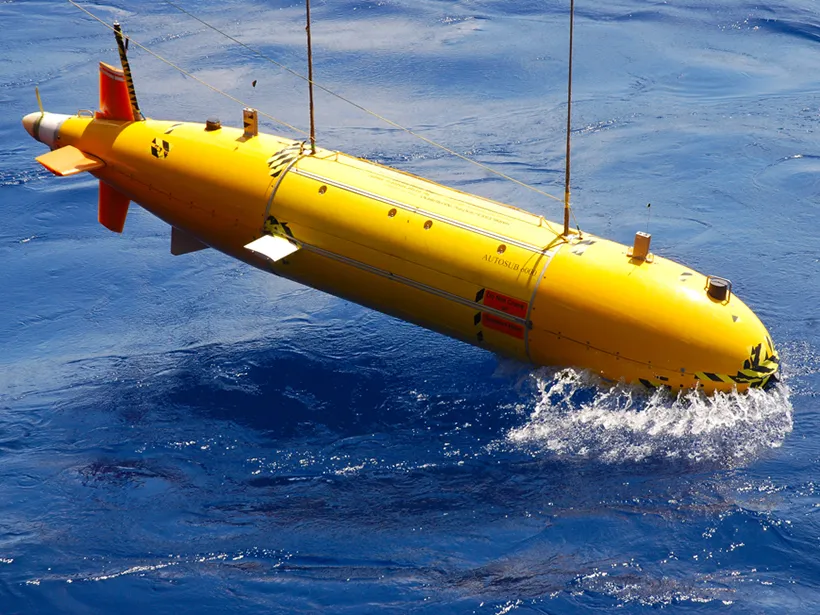
\includegraphics[height = 2.5cm, width=0.3\textwidth]{AUV_2.png}
        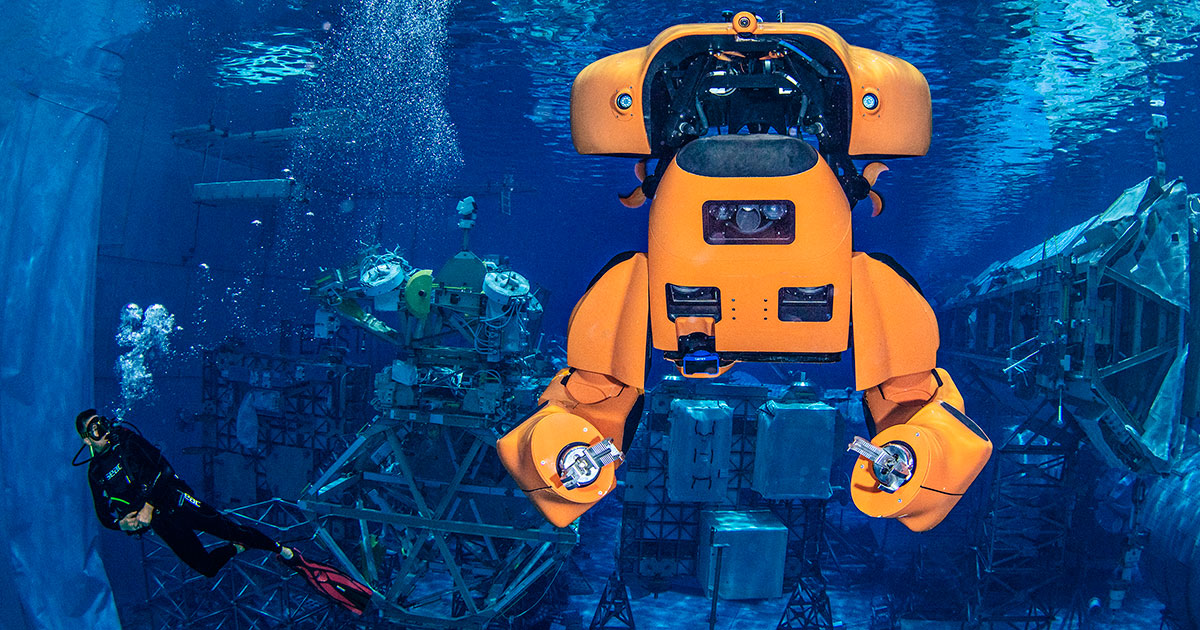
\includegraphics[height = 2.5cm, width=0.3\textwidth]{aquanaut.jpg}
        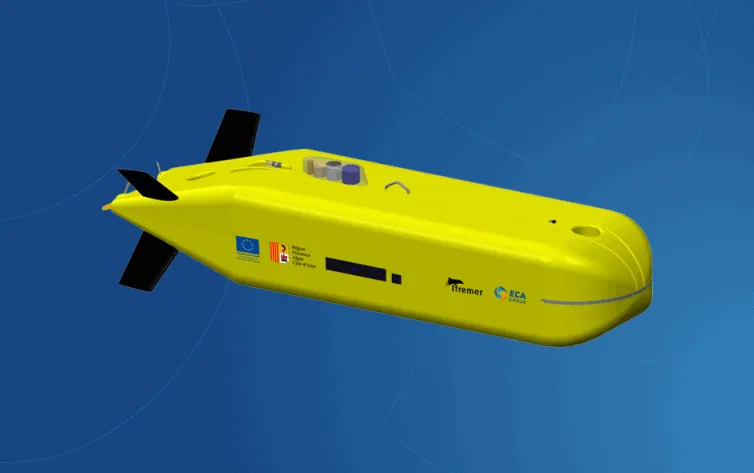
\includegraphics[height = 2.5cm, width=0.3\textwidth]{auv-3.png}
    
    \end{figure}
    
%*----------- notes
    \note[item]{Notes can help you to remember important information. Turn on the notes option.}
\end{frame}
%-
%*----------- SLIDE -------------------------------------------------------------
\begin{frame}[c]{Problema de pesquisa} 
    \transdissolve[duration=0.5]
   
    \begin{center}
        \Wider{%
        \begin{shaded}
        \begin{center}
            \vspace*{0.4cm}
            \resizebox{!}{1.3cm}{%
               % \color{bg} O objetivo é ter um objetivo.
                \begin{tabular}{ccc}
                    De que forma as forças hidrodinâmicas podem \\
                    afetar e impactar na navegação de um sistema  \\ 
                    robótico submarino?      
                  \end{tabular}
            }%
        \end{center}
        \end{shaded}
        }%
    \end{center}
%*----------- notes
    \note[item]{Notes can help you to remember important information. Turn on the notes option.}
\end{frame}
%-
%*----------- SLIDE -------------------------------------------------------------
\begin{frame}[t]{Objetivos}
    Objetivo Geral
    \newline
    Desenvolver um modelo de veículo submarino para a navegação em águas rasas.
    \newline

    Objetivos Específicos
    \begin{itemize}
        \item Realizar o estudo do estado da arte
        \item Realizar o desing da estrutura do submarino
        \item Realizae simuolações (CFD,ROS)
        \item Desenvolver o planejamento dos experimentos
        \item Desenvolver artigos científicos
    \end{itemize}

%*----------- notes
    \note[item]{Notes can help you to remember important information. Turn on the notes option.}
\end{frame}
%-
%*----------- SLIDE -------------------------------------------------------------
\begin{frame}[t]{Referencial Teórico}
\vspace{0.5cm}
     \begin{table}[ht!]
    \centering
        \caption{}
            \begin{tabular}{|c|c|c|} \hline
             \textbf{Tema}&\textbf{Autor}\\ \hline
             Underwater Robotics & Gianluca Antonelli(2014)\\ \hline
             A review paper on: Autonomous underwater vehicle & Sandeep Kumar Jain et al.(2015) \\ \hline
             Hybrid Underwater Robot System Based on ROS & Abdou Y. M. Sani et al. (2019)\\ \hline
         \end{tabular}
     \end{table}

%*----------- notes
\note[item]{Notes can help you to remember important information. Turn on the notes option.}
\end{frame}
%-
%*----------- SLIDE -------------------------------------------------------------
\begin{frame}[c]{Metodologia }
    %\transboxin[duration=1,direction=30]
        \begin{figure}
        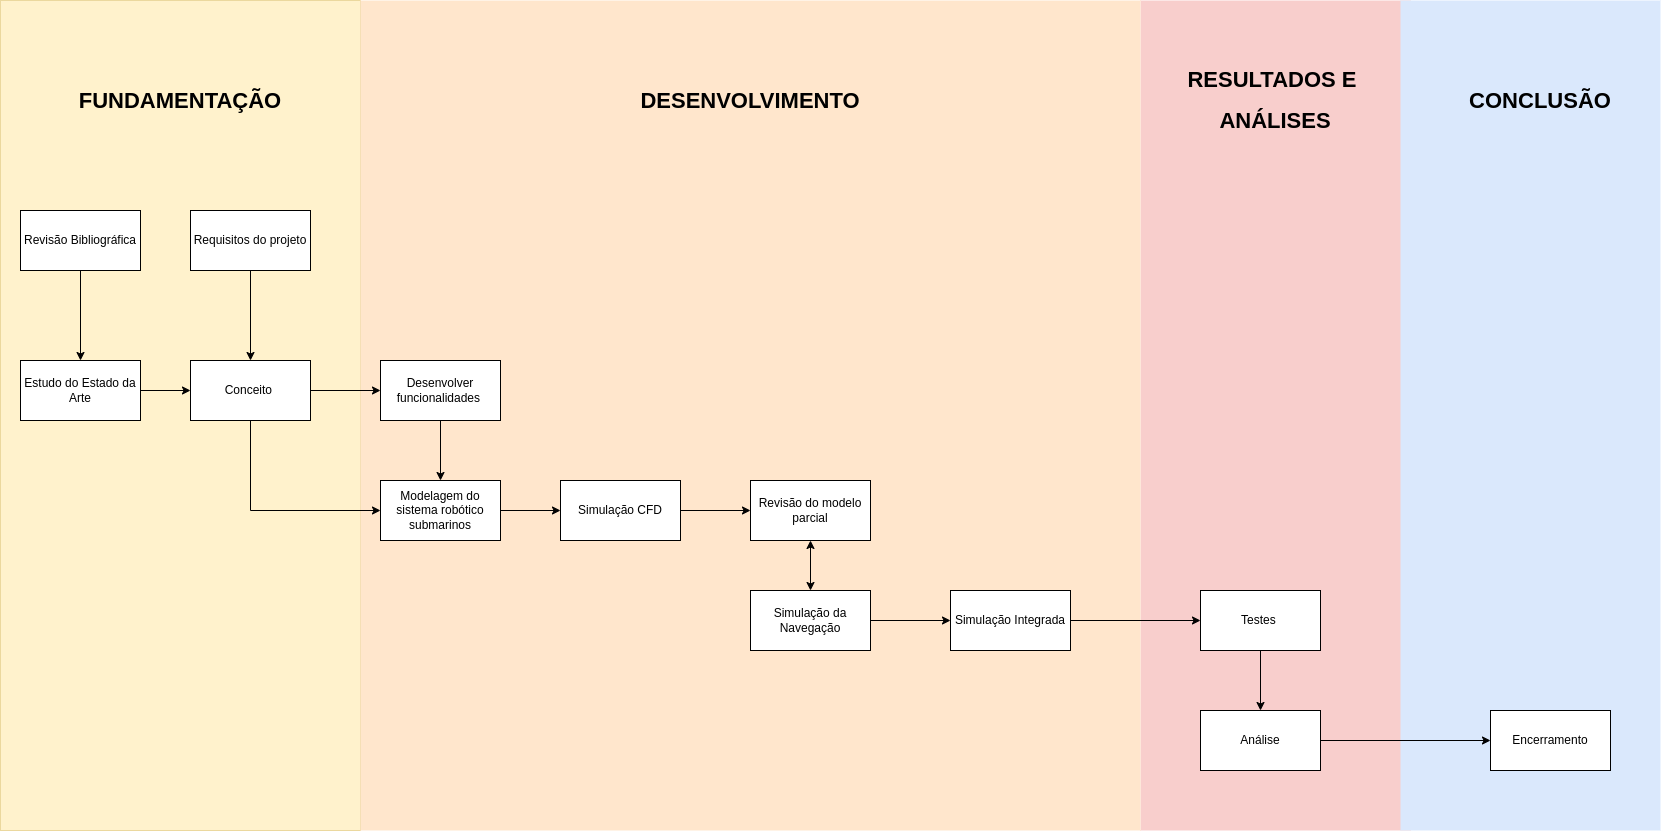
\includegraphics[width=.9\textwidth]{metodologiamodi1.png}
    \end{figure}
%*----------- notes
    \note[item]{Notes can help you to remember important information. Turn on the notes option.}
\end{frame}
%-
%*----------- SLIDE -------------------------------------------------------------
\begin{frame}[c]{Metodo BiLi}
    %\transboxin[duration=1,direction=30]
        \begin{figure}
        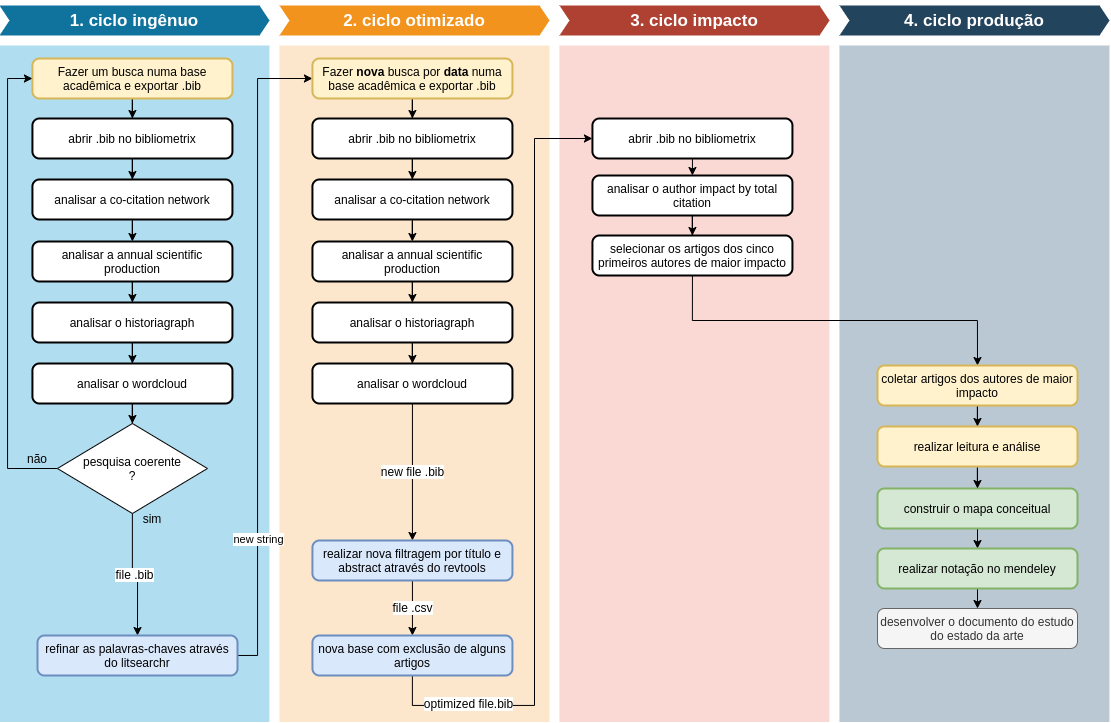
\includegraphics[width=.7\textwidth]{bili.png}
    \end{figure}
%*----------- notes
    \note[item]{Notes can help you to remember important information. Turn on the notes option.}
\end{frame}
%-
% %*----------- SLIDE -------------------------------------------------------------
% \begin{frame}[t]{Método BiLi}
%     \textbf{Ciclo Ingênuo} 
%     \newline
%         Foram pesquisados 10 ".bib" para chegar no resultado 
%     \newline
%         Palavras chaves: underwater vehicle,underwater robotics,cfd modeling,cfd simulation, OpenFOAM
%     \newline
%         Artigos encontrados: 633
%     \newline
%         String gereada: "underwater vehicle" OR "autonomous underwater" OR "operated vehicle" OR
%         "remotely operated" OR "robotic vehicle" OR "underwater robot") AND ("computational fluid" OR "fluid dynamic") 
%         AND ("control system" OR "fluid dynamics")
%     \newline
%     \textbf{Ciclo Otmizado}
%     \newline
%         Utilização do litserach para otimização da strin
%     \newline
%         Artigos encontrados: 733
%     \newline
%         Filtragem do RevTools: 357 artigos

% %*----------- notes
%     \note[item]{Notes can help you to remember important information. Turn on the notes option.}
% \end{frame}
% %-
% *----------- SLIDE -------------------------------------------------------------
\begin{frame}[t]{Ciclo Ingênuo X Ciclo Otmizado}
    \transboxout[duration=0.5]
    \framesubtitle{Taxa de crescimento anual de artigos científicos}
    
    \begin{columns}
        \column{.4\textwidth}
        \newline  
            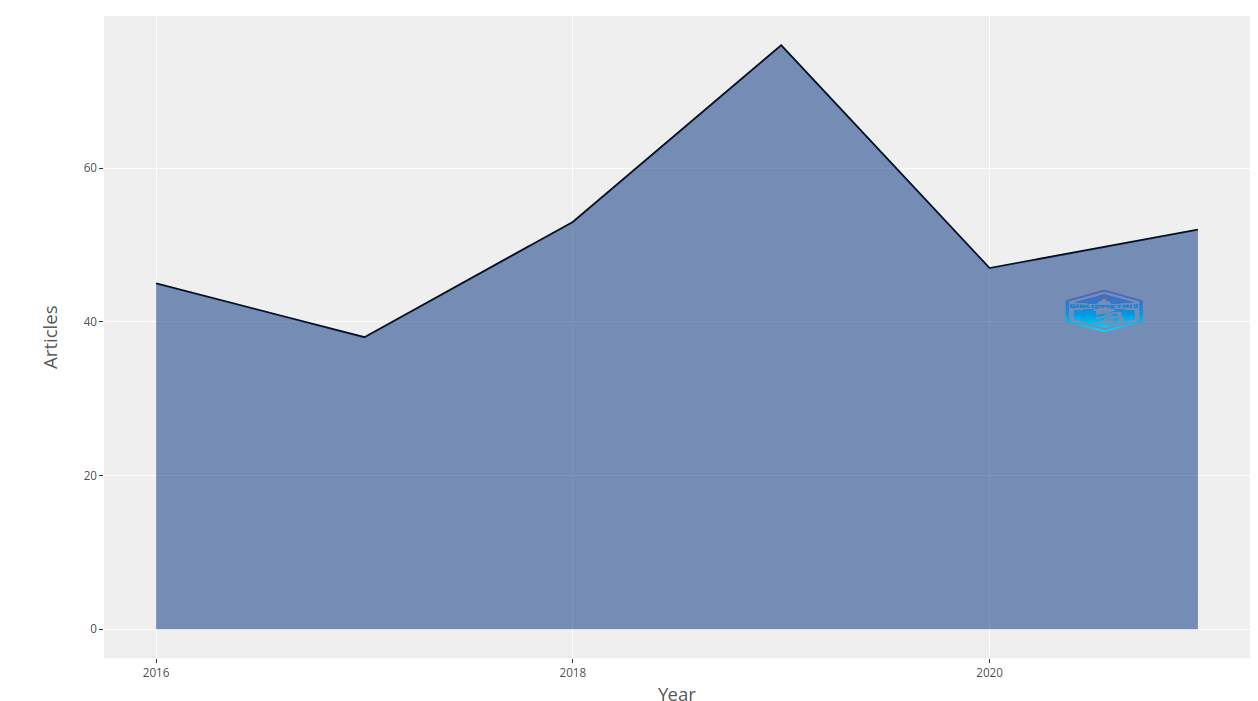
\includegraphics[height = 4cm, width=1.2\textwidth]{produçãoanual1.png}
        \column{.4\textwidth}
        \newline  
         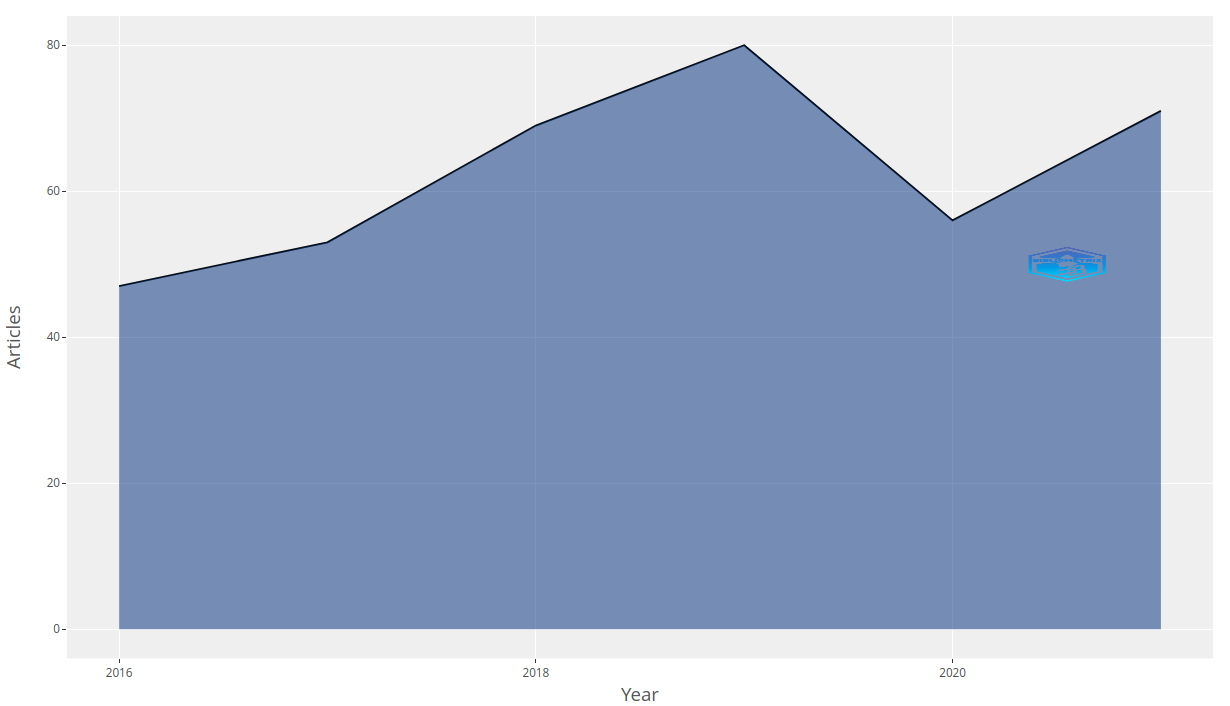
\includegraphics[height = 4cm, width=1.2\textwidth]{producaanual2.png}
    \end{columns}
    
    \begin{columns}
        \column{.4\textwidth}
        \newline  
        Taxa de crescimento: 2.93\%
        \column{.4\textwidth}
        \newline
         Taxa de crescimento: 8.6\%
    \end{columns}
 %*----------- notes
    \note[item]{Notes can help you to remember important information. Turn on the notes option.}
\end{frame}
%-
% *----------- SLIDE -------------------------------------------------------------
\begin{frame}[t]{Ciclo Ingênuo X Ciclo Otmizado}
    \transboxout[duration=0.5]
    \framesubtitle{Rede de co-citação}
    
    \begin{columns}
        \column{.4\textwidth}
        \newline  
            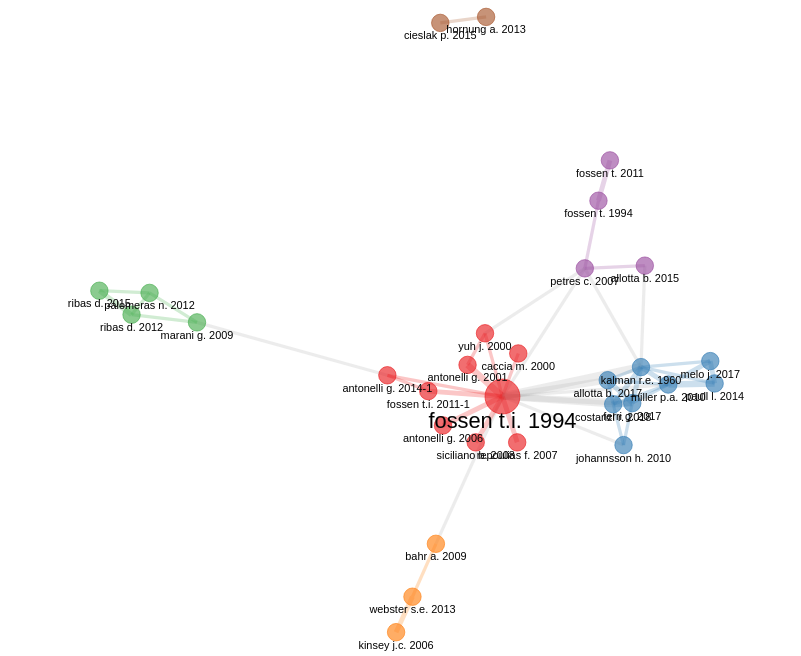
\includegraphics[height = 5cm, width=1.2\textwidth]{cocitação1.png}
        \column{.4\textwidth}
        \newline  
         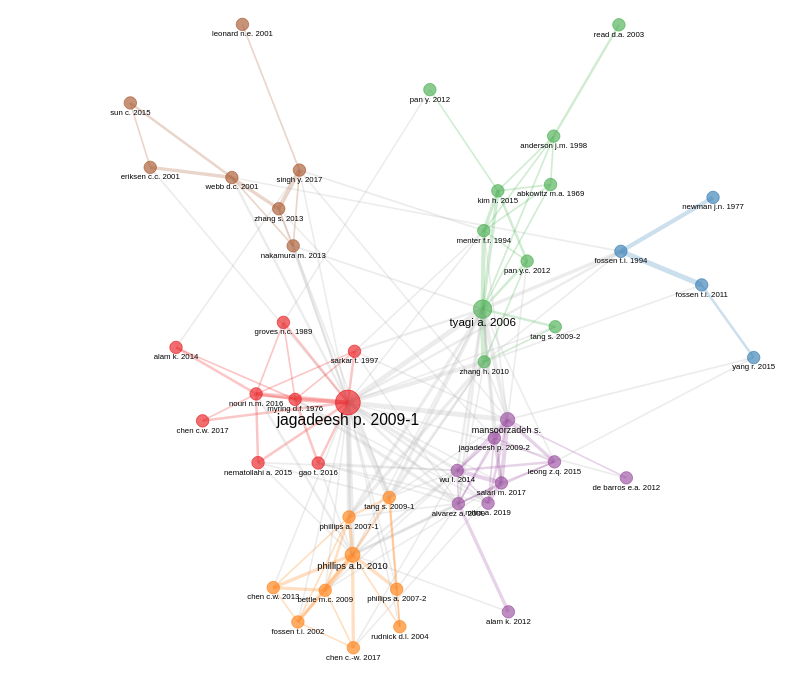
\includegraphics[height = 5cm, width=1.2\textwidth]{cocitação2.png}
    \end{columns}
    
 %*----------- notes
    \note[item]{Notes can help you to remember important information. Turn on the notes option.}
\end{frame}
%-
% *----------- SLIDE -------------------------------------------------------------
\begin{frame}[t]{Ciclo Ingênuo X Ciclo Otmizado}
    \transboxout[duration=0.5]
    \framesubtitle{Mapa de palavras}
    
    \begin{columns}
        \column{.4\textwidth}
        \newline  
            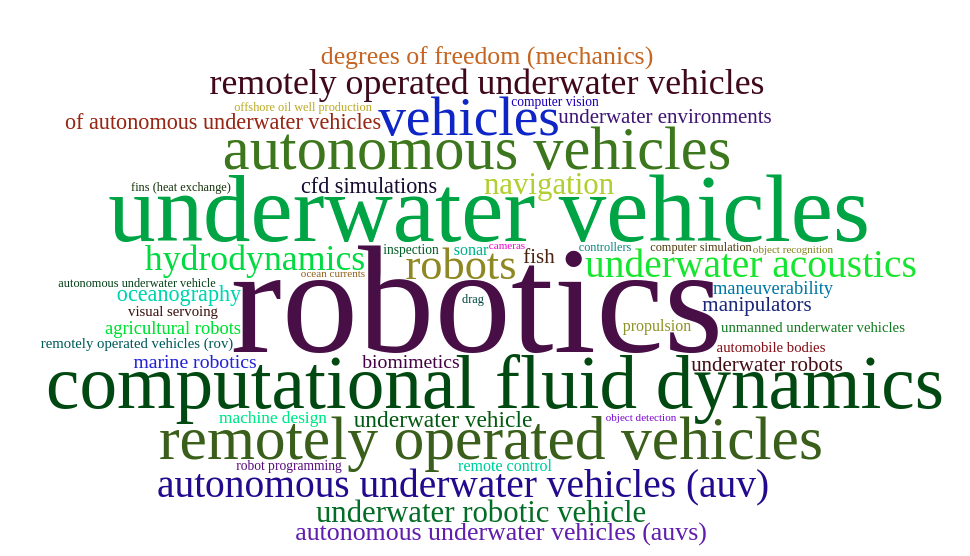
\includegraphics[height = 4cm, width=1.2\textwidth]{mapadepalavras1.png}
        \column{.4\textwidth}
        \newline  
         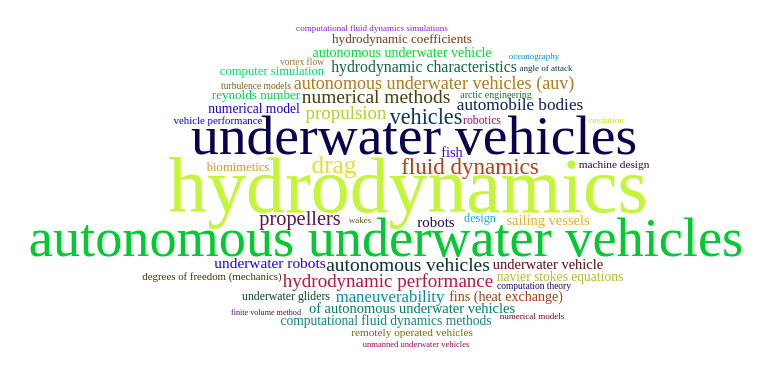
\includegraphics[height = 4cm, width=1.2\textwidth]{mapadepalavras2.png}
    \end{columns}
    
 %*----------- notes
    \note[item]{Notes can help you to remember important information. Turn on the notes option.}
\end{frame}
%-
%*----------- SLIDE -------------------------------------------------------------
\begin{frame}[c]{Resultados esperados}
    \begin{itemize}
        \item Um veículo submarino capaz de se locomover de forma autonôma e consiga realizar inspeção 
        nas regiões subaquáticas
        
    \end{itemize}

    \begin{figure}
        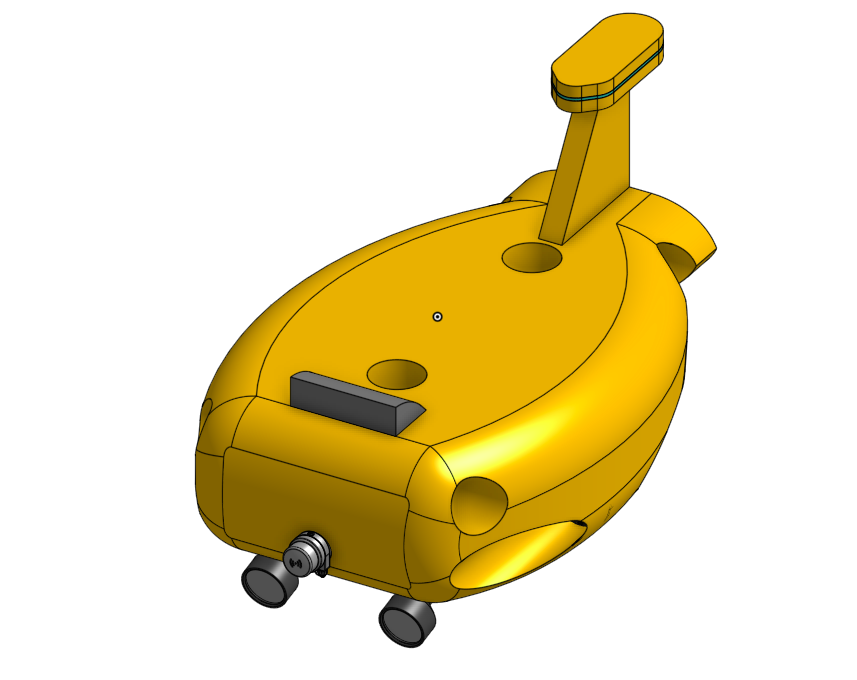
\includegraphics[trim = 0 20 0 50, clip, width=0.4\textwidth]{turbot-fish-01modi.png}
        %\caption{.}
    \end{figure}
%*----------- notes
    \note[item]{Notes can help you to remember important information. Turn on the notes option.}
\end{frame}
%-
%*----------- SLIDE -------------------------------------------------------------
\begin{frame}[c]{}
    \begin{center}
        \Wider{%
        \begin{shaded}
        \begin{center}
            \vspace*{0.8cm}
            \resizebox{!}{1cm}{%
               % \color{bg} O objetivo é ter um objetivo.
                \begin{tabular}{ccc}
                    \textbf{Principais Aprendizados}   
                  \end{tabular}
            }%
        \end{center}
        \end{shaded}
        }%
    \end{center}
%*----------- notes
    \note[item]{Notes can help you to remember important information. Turn on the notes option.}
\end{frame}
%-
